% Provenance (never printed): see sources/outline_sources.md (Year 1: litho-, bio- and
% chronostratigraphy; boundary stratotypes; mass extinctions as global markers; the
% international chart). Exercise and problem values in the Book 3 scratch calculator
% calc/ch24.py; the chart from figdata/bachelor-1/ics_chart.py (shared ics rows).
% The principles of relative dating, eras and periods are Book 1's (g7 geological-time) and
% are re-founded here. Mass extinctions belong to the biology series (recalled in prose);
% their Earth causes are the Year 2 volume's (phanerozoic-earth). Correlation of logs and
% unconformities are ch. 5's; facies ch. 21's; compaction ch. 23's. Radiometric dating is
% ch. 25's. Sequence stratigraphy, facies models and Walther's law are the Year 3 volume's;
% magnetostratigraphy too: prose pointers only. "Transgression" is explained in prose.
\chapter{La escala estratigráfica}\label{ch:b1:stratigraphic-scale}

En la playa de Itzurun, en Zumaia, en la costa vasca, los acantilados están hechos de capas finas de caliza y marga, inclinadas y repetidas durante cientos de metros. En un contacto, donde una capa
de caliza pálida termina y empiezan unas margas rojas, está incrustado en la roca un disco de bronce marcado con cuatro letras (figura de abajo). Es un clavo de oro. Fija, para todo el planeta, el
instante en que empieza una división del tiempo geológico --- el \omterm{def:b1:stratigraphic-scale:chronostratigraphy}{piso} Selandiense. Una roca de la Patagonia o de Siberia es selandiense si se depositó después del instante registrado en ese
contacto y antes del que registra el siguiente clavo más arriba en la escala. Este capítulo explica cómo los geólogos llegaron a necesitar tal marcador: tres formas distintas de dividir una pila de
rocas, los principios que las ordenan, las líneas que unen secciones alejadas, y la carta internacional que recoge el resultado.

\begin{omfigure}
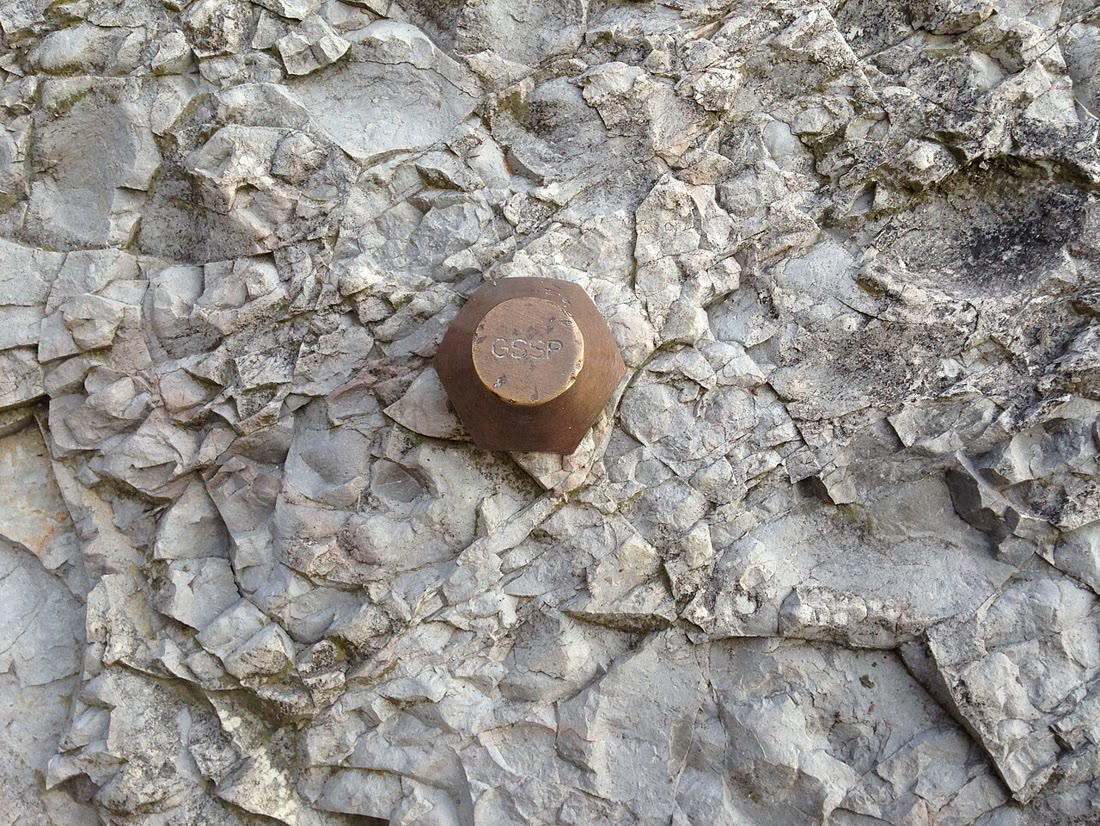
\includegraphics[width=0.62\linewidth]{images/book3/b1-golden-spike-zumaia.jpg}

{\small El clavo de oro del \omterm{def:b1:stratigraphic-scale:chronostratigraphy}{piso} Selandiense en la sección de Zumaia: un marcador de bronce marcado GSSP, colocado en la cima de la capa de caliza más alta de una \omterm{def:b1:stratigraphic-scale:lithostratigraphy}{formación}, en la base de las
margas rojas de la siguiente. (Josugoni, CC~BY-SA~4.0, a través de Wikimedia Commons.)}
\label{fig:b1:stratigraphic-scale:zumaia}
\end{omfigure}
% ledger: commons:zumaia-gssp, gssp:selandian

\begin{recall}
En una pila de capas que no se ha volcado, cada capa es más joven que la de debajo; una estructura que corta las rocas es más joven que ellas; los fósiles cambian de las capas más antiguas a
las más jóvenes en el mismo orden en todas partes; la historia de la Tierra se divide en eras y períodos geológicos, cada uno con una edad en años para su inicio, reunidos en una carta internacional
(libro 1, año 7). Un \omterm{def:b1:cross-sections:log}{registro de sondeo} anota las unidades encontradas según la profundidad, y la correlación empareja las mismas unidades de un registro a otro (\cref{def:b1:cross-sections:log});
una \omterm{def:b1:cross-sections:unconformity}{discordancia} es una superficie de erosión o de no depósito (\cref{def:b1:cross-sections:unconformity}). Una \omterm{def:b1:clastic-sediments:facies}{facies sedimentaria} es un cuerpo de roca cuyos caracteres registran su ambiente de depósito
(\cref{def:b1:clastic-sediments:facies}). Los volúmenes de biología describen cómo aparecen y se extinguen las especies, y las pocas extinciones masivas en las que una gran parte de todas las especies
desapareció en un intervalo corto de tiempo.
\end{recall}

\section{Tres formas de dividir las rocas}\label{sec:b1:stratigraphic-scale:three}

Un geólogo que levanta un perfil de un acantilado puede dividir la misma pila de estratos de tres maneras: según de qué están hechas las rocas, según los fósiles que contienen, y según el tiempo
en el que se depositaron. Las tres divisiones responden a preguntas distintas, y sus límites no tienen por qué coincidir. Las reglas para nombrar y definir cada clase de unidad se fijan por acuerdo internacional.
% ledger: isg:lithostratigraphy

\begin{definition}[Formación, miembro, grupo]\label{def:b1:stratigraphic-scale:lithostratigraphy}
Una \emph{unidad litoestratigráfica}\index{unidad litoestratigráfica} es un cuerpo de roca definido y reconocido por su litología y por su posición entre otros cuerpos, sea cual sea su edad. La unidad
primaria es la \emph{formación}\index{formación (litoestratigráfica)}: un cuerpo de roca lo bastante distinto de sus vecinos como para cartografiarlo a escala regional, en el que debe dividirse toda la columna.
Un \emph{miembro}\index{miembro (litoestratigráfico)} es una subdivisión con nombre de una formación, distinguida por su litología; un \emph{grupo}\index{grupo (litoestratigráfico)} es una sucesión de dos
o más formaciones con caracteres litológicos significativos en común. Un nombre formal une un nombre geográfico local con el rango o con la roca dominante: la Arenisca de Kell, la Formación de Lutita de Mardon.
\end{definition}
% ledger: isg:lithostratigraphy

Una \omterm{def:b1:stratigraphic-scale:lithostratigraphy}{formación} puede tener menos de un metro de espesor o varios miles de metros. Se extiende lejos de su sección tipo solo hasta donde puede reconocerse su litología, así que sus límites siguen la roca, no el tiempo.
% ledger: isg:lithostratigraphy

\begin{definition}[Biozona, fósil guía, datum de primera aparición]\label{def:b1:stratigraphic-scale:biozone}
Una \emph{biozona}\index{biozona} es un cuerpo de estratos definido o caracterizado por los fósiles que contiene. Una \emph{zona de rango}\index{zona de rango} reúne las apariciones conocidas de un taxón;
una \emph{zona de intervalo}\index{zona de intervalo} es el cuerpo de estratos comprendido entre dos horizontes fósiles especificados, por ejemplo las apariciones más bajas de dos taxones. El \emph{datum de primera aparición}\index{datum de primera aparición}
(FAD) de un taxón es el horizonte de su aparición más baja, el \emph{datum de última aparición}\index{datum de última aparición} el de la más alta. Un \emph{fósil guía}\index{fósil guía} es un taxón usado para
reconocer una biozona: los mejores son extendidos, abundantes, fáciles de identificar y de vida corta.
\end{definition}
% ledger: isg:biostratigraphy, og:stratigraphy-principles

Un horizonte fósil no tiene espesor; una \omterm{def:b1:stratigraphic-scale:biozone}{biozona} puede tener unos metros o unos cientos de metros de espesor según la rapidez con que se acumuló el sedimento mientras vivían los taxones. Como las especies evolucionan
y no reaparecen una vez extinguidas, el conjunto de fósiles de una edad cualquiera es único. Algunos de los mejores \omterm{def:b1:stratigraphic-scale:biozone}{fósiles guía} son microfósiles, como los foraminíferos y los conodontos: extendidos, abundantes y lo bastante pequeños
para recuperarse de los recortes de un pozo.
% ledger: isg:biostratigraphy, og:stratigraphy-principles

\begin{definition}[Unidades cronoestratigráficas y geocronológicas]\label{def:b1:stratigraphic-scale:chronostratigraphy}
Una \emph{unidad cronoestratigráfica}\index{unidad cronoestratigráfica} es el cuerpo de todas las rocas formadas durante un intervalo dado de tiempo geológico, y solo durante él; sus límites son superficies de igual edad.
El intervalo de tiempo en sí es una \emph{unidad geocronológica}\index{unidad geocronológica}. Los rangos, de menor a mayor, son el \emph{piso}\index{piso (cronoestratigráfico)} (su tiempo: una edad), la \emph{serie}\index{serie (cronoestratigráfica)}
(una época), el \emph{sistema}\index{sistema (cronoestratigráfico)} (un período), el eratema (una era) y el eonotema (un eón); cada unidad está hecha de varias unidades consecutivas del rango inferior.
\end{definition}
% ledger: isg:chronostratigraphy

Las dos palabras describen la misma división vista como roca o como tiempo (\cref{tab:b1:stratigraphic-scale:ranks}): las rocas del \omterm{def:b1:stratigraphic-scale:chronostratigraphy}{Sistema} Jurásico se depositaron durante el Período Jurásico, y la \omterm{def:b1:stratigraphic-scale:chronostratigraphy}{Serie} Jurásica Inferior durante la Época del Jurásico Temprano. El \omterm{def:b1:stratigraphic-scale:chronostratigraphy}{piso} es la unidad más pequeña reconocida en todo el mundo.
% ledger: isg:chronostratigraphy, chart:danian

\begin{table}[htbp]
\centering
\begin{tabular}{lll}
\hline
\shortstack[l]{\omterm{def:b1:stratigraphic-scale:chronostratigraphy}{unidad cronoestratigráfica}\\(roca)} & \shortstack[l]{\omterm{def:b1:stratigraphic-scale:chronostratigraphy}{unidad geocronológica}\\(tiempo)} & ejemplo \\
\hline
eonotema & eón    & Fanerozoico \\
eratema  & era    & Cenozoico \\
\omterm{def:b1:stratigraphic-scale:chronostratigraphy}{sistema}   & período & Paleógeno \\
\omterm{def:b1:stratigraphic-scale:chronostratigraphy}{serie}   & época  & Paleoceno \\
\omterm{def:b1:stratigraphic-scale:chronostratigraphy}{piso}    & edad    & Daniense (\qtyrange{66.00}{61.66}{\Ma}) \\
\hline
\end{tabular}
\caption{Los rangos de las \omterm{def:b1:stratigraphic-scale:chronostratigraphy}{unidades cronoestratigráficas} y geocronológicas, con las unidades que contienen el Daniense, el primer \omterm{def:b1:stratigraphic-scale:chronostratigraphy}{piso} del Cenozoico.}
\label{tab:b1:stratigraphic-scale:ranks}
\end{table}
% ledger: isg:chronostratigraphy, chart:danian

\section{Los principios y la correlación}\label{sec:b1:stratigraphic-scale:principles}

Antes de que ninguna roca pudiera fecharse en años, el orden de los sucesos se leyó en las propias rocas. Los principios básicos de la estratigrafía los expuso en 1669 Nicolás Steno; entre 1785 y 1800 Hutton y William Smith añadieron el uso de los estratos como intervalos de tiempo y de sus fósiles para reconocerlos.
% ledger: og:stratigraphy-principles, usgs:hutton-smith

\begin{definition}[Principios de la estratigrafía]\label{def:b1:stratigraphic-scale:principles}
\begin{enumerate}
  \item El \emph{principio de superposición}\index{superposición, principio de}: en una sucesión de capas sedimentarias que no se ha volcado, cada capa es más joven que aquella sobre la que descansa.
  \item El \emph{principio de horizontalidad original}\index{horizontalidad original, principio de}: los sedimentos y las coladas de lava se depositan horizontales, o casi --- ligeramente inclinados en los bordes de una cuenca.
  \item El \emph{principio de continuidad lateral}\index{continuidad lateral, principio de}: dentro de una cuenca, una capa se extiende sin interrupción en todas las direcciones hasta adelgazarse en el borde de la cuenca o contra un obstáculo; una capa cortada por un valle continúa al otro lado.
  \item El \emph{principio de las relaciones de corte}\index{relaciones de corte, principio de}: un cuerpo o estructura que corta las rocas --- un dique, una falla, una superficie de erosión --- es más joven que las rocas que corta.
  \item El \emph{principio de sucesión faunística}\index{sucesión faunística, principio de}: los taxones fósiles se suceden unos a otros en el mismo orden en todas las regiones, de modo que las rocas que contienen el mismo conjunto son de la misma edad.
\end{enumerate}
\end{definition}
% ledger: og:stratigraphy-principles, eli:relative-dating, usgs:fossil-succession, isg:chronostratigraphy

Los principios no son igual de fuertes. La superposición da un orden que todo otro método debe respetar. La horizontalidad original es lo que hace de un estrato inclinado un registro de deformación posterior. La continuidad lateral es lo que permite a un geólogo dibujar la misma capa a ambos lados de un valle, y, dentro de una distancia limitada, un plano de estratificación trazado sobre el terreno es la mejor línea de igual edad que hay. La sucesión faunística es la que cruza los océanos; es el tema de los párrafos siguientes.
% ledger: isg:chronostratigraphy, og:stratigraphy-principles

\subsection*{Correlación mediante biozonas}

La correlación por fósiles compara el orden de las primeras y últimas apariciones en dos secciones (figura de abajo). Las dos no son igual de fiables. El fósil más alto de un taxón hallado en una sección depende de cuántos se conservaron: donde son raros, el último hallado puede yacer muy por debajo del nivel en que el taxón desapareció de verdad, y un fósil erosionado y vuelto a depositar puede aparecer por encima de él. Una primera aparición también puede desplazarse, pero un taxón extendido que se difundió deprisa se alcanza aproximadamente al mismo nivel a lo ancho de una cuenca.
% ledger: isg:biostratigraphy

\begin{omfigure}
\begin{tikzpicture}[font=\footnotesize, y=0.13cm]
  % section 1: 40 m, sandstone 0-14, shale 14-40
  \fill[lith sandstone] (0,0) rectangle (0.8,14);
  \fill[lith shale] (0,14) rectangle (0.8,40);
  \draw[black!70] (0,0) rectangle (0.8,40);
  \node[anchor=south, font=\small] at (1.4,41.5) {sección 1};
  \foreach \x/\a/\b/\t in {1.1/0/27/a, 1.4/10/34/b, 1.7/20/40/c, 2.0/30/40/d} {
    \draw[line width=2.2pt, omThm] (\x,\a) -- (\x,\b);
    \node[anchor=base, font=\scriptsize] at (\x,-4.5) {\t};
  }
  \foreach \y/\z in {5/a, 15/b, 25/c, 35/d}
  \node[anchor=east, font=\scriptsize] at (-0.1,\y) {zona \z};
  \foreach \y in {10,20,30} \draw[black!50] (-1.3,\y) -- (0,\y);
  % scale bar
  \draw[thick] (-1.5,0) -- (-1.5,10) node[midway, anchor=east, font=\scriptsize] {\qty{10}{m}};
  % section 2: 24 m, sandstone 0-3, shale 3-24
  \begin{scope}[xshift=7cm]
    \fill[lith sandstone] (0,0) rectangle (0.8,3);
    \fill[lith shale] (0,3) rectangle (0.8,24);
    \draw[black!70] (0,0) rectangle (0.8,24);
    \node[anchor=south, font=\small] at (1.4,25.5) {sección 2};
    \foreach \x/\a/\b/\t in {1.1/0/13/a, 1.4/6/20/b, 1.7/12/24/c, 2.0/18/24/d} {
      \draw[line width=2.2pt, omThm] (\x,\a) -- (\x,\b);
      \node[anchor=base, font=\scriptsize] at (\x,-4.5) {\t};
    }
    \foreach \y/\z in {3/a, 9/b, 15/c, 21/d}
      \node[anchor=west, font=\scriptsize] at (2.3,\y) {zona \z};
    \foreach \y in {6,12,18} \draw[black!50] (0.8,\y) -- (2.3,\y);
  \end{scope}
  % correlation of the first appearances
  \foreach \u/\v/\t in {10/6/b, 20/12/c, 30/18/d}
    \draw[densely dashed, omThm!70!black] (2.15,\u) -- (6.85,\v)
      node[pos=0.5, fill=white, inner sep=1pt, font=\scriptsize] {FAD \t};
\end{tikzpicture}

{\small Un diagrama de rangos y una correlación por \omterm{def:b1:stratigraphic-scale:biozone}{biozonas} (taxones inventados \emph{a} a \emph{d}). Las barras gruesas son los rangos de los taxones en cada sección. Tres \omterm{def:b1:stratigraphic-scale:biozone}{zonas de
intervalo} están limitadas por las primeras apariciones de \emph{b}, \emph{c} y \emph{d}, que se unen de una sección a otra (discontinuas). La última aparición de \emph{a} cae en la parte
alta de la zona~\emph{c} en la sección~1 y cerca de su base en la sección~2: es una guía peor. Las zonas son más delgadas en la sección~2, donde el sedimento se acumuló más despacio.}
\label{fig:b1:stratigraphic-scale:range-chart}
\end{omfigure}

\begin{method}[Correlacionar secciones mediante biozonas]\label{met:b1:stratigraphic-scale:biozones}
\begin{enumerate}
  \item Represéntese, para cada sección, el rango de cada taxón frente a la altura: desde su aparición más baja hasta la más alta.
  \item Elíjanse los horizontes fósiles que definen las zonas, preferiblemente primeras apariciones de taxones extendidos que sean independientes de la facies.
  \item Trácense los límites de zona en cada sección en estos horizontes.
  \item Únanse de una sección a otra los mismos horizontes; compruébese que las líneas no se cruzan, como exige la superposición.
  \item Léase, entre dos líneas, el espesor de cada zona en cada sección; donde falte una zona, búsquese una \omterm{def:b1:cross-sections:unconformity}{discordancia} o un cambio de facies antes de concluir que el taxón está ausente.
\end{enumerate}
\end{method}

Una \omterm{def:b1:stratigraphic-scale:biozone}{biozona} solo es tan buena como la independencia de sus fósiles respecto del ambiente. Un bivalvo que vivió solo en orillas arenosas se encuentra solo en areniscas; seguirlo de sección en sección sigue a la arenisca, no al tiempo. La correlación bioestratigráfica no es, pues, necesariamente una correlación temporal: puede seguir una facies cuya edad cambia de un lugar a otro.
% ledger: isg:biostratigraphy

\subsection*{Límites que cruzan el tiempo}

Distintos sedimentos se depositan al mismo tiempo en lugares distintos: arena en la orilla, lodo mar adentro, caliza más lejos en una plataforma sin arena. Una línea de igual edad pasa, pues, de una litología a otra. A la inversa, un límite litológico trazado a lo ancho de una cuenca no tiene por qué ser en absoluto una línea de igual edad.
% ledger: og:stratigraphy-principles, isg:chronostratigraphy

\begin{definition}[Límite diacrónico]\label{def:b1:stratigraphic-scale:diachronous}
Un límite es \emph{diacrónico}\index{límite diacrónico} cuando su edad cambia de un lugar a otro a lo largo de él. Los límites de formaciones y de facies suelen ser diacrónicos; los límites de las \omterm{def:b1:stratigraphic-scale:chronostratigraphy}{unidades cronoestratigráficas} no lo son, por definición.
\end{definition}
% ledger: isg:lithostratigraphy, isg:chronostratigraphy, isg:biostratigraphy

El caso clásico es una transgresión: el \omterm{def:b1:diagenesis-basins:eustasy}{nivel relativo del mar} sube más deprisa de lo que el sedimento puede llenar el espacio creado, y la línea de costa se desplaza tierra adentro. La arena de playa se deposita en la línea de costa en cada instante, así que una capa de arenisca se extiende tierra adentro con ella; el lodo de mar adentro la sigue por encima. La cima de la arenisca es entonces la traza de la línea de costa en movimiento: joven tierra adentro, vieja mar adentro (figura de abajo). El orden de las facies visto en una sección vertical --- arenisca bajo lutita bajo caliza --- repite su orden a lo ancho de la plataforma en un instante; el volumen del año~3 hace de esto la base de sus modelos de facies.
% ledger: og:stratigraphy-principles, isg:lithostratigraphy

\begin{omfigure}
\begin{tikzpicture}[font=\footnotesize, x=1cm, y=1cm]
  % basement surface B(x) = 1.6 (1 - x/14), rising towards the land on the left
  \fill[lith granite] (0,-0.5) -- (0,1.6) -- (14,0) -- (14,-0.5) -- cycle;
  \fill[lith sandstone] (0,1.6) -- (14,0) -- (14,0.5) -- (0,2.1) -- cycle;
  \fill[lith shale] (0,2.1) -- (14,0.5) -- (14,1.5) -- (0,3.1) -- cycle;
  \fill[lith limestone] (0,3.1) -- (14,1.5) -- (14,3.6) -- (0,3.6) -- cycle;
  \draw[unconformity] (0,1.6) -- (14,0);
  \draw[black!70] (0,2.1) -- (14,0.5) (0,3.1) -- (14,1.5);
  \draw[black!70] (0,-0.5) rectangle (14,3.6);
  % time lines: horizontal, from the basement (or the left edge) to the right edge
  \foreach \y/\t in {0.6/1, 1.1/2, 1.6/3, 2.1/4, 2.6/5, 3.1/6} {
    \pgfmathsetmacro{\xs}{max(0, 14*(1-\y/1.6))}
    \draw[omThm, thick, densely dashed] (\xs,\y) -- (14,\y) node[anchor=west, text=black] {$t_\t$};
  }
  % two sections
  \foreach \x/\n in {3/1, 11/2} {
    \draw[very thick, black] (\x,-0.5) -- (\x,3.6);
    \node[anchor=south, font=\small] at (\x,3.65) {sección \n};
  }
  \node[fill=white, inner sep=1pt, font=\scriptsize] at (5.6,1.21) {arenisca};
  \node[fill=white, inner sep=1pt] at (12.6,1.2) {lutita};
  \node[fill=white, inner sep=1pt] at (7.0,3.25) {caliza};
  \node[fill=white, inner sep=1pt] at (12.0,-0.25) {basamento};
  \draw[-{Stealth}, thick] (5.6,4.35) -- (3.6,4.35) node[anchor=east] {tierra};
  \draw[-{Stealth}, thick] (8.4,4.35) -- (10.4,4.35) node[anchor=west] {mar};
\end{tikzpicture}

{\small Una lámina de arenisca depositada durante una transgresión (esquemático, escala vertical exagerada). Las líneas discontinuas $t_1$ a $t_6$ unen puntos de igual edad,
siendo $t_1$ la más antigua. Donde una de ellas se encuentra con el basamento, empieza en la línea de costa de su tiempo; mar adentro pasa de arena a lodo y, en las más jóvenes, a caliza.
La cima de la arenisca yace entre $t_1$ y $t_2$ en la sección~2, pero entre $t_3$ y $t_4$ en la sección~1: el límite de la \omterm{def:b1:stratigraphic-scale:lithostratigraphy}{formación} es \omterm{def:b1:stratigraphic-scale:diachronous}{diacrónico}, más joven hacia la tierra.}
\label{fig:b1:stratigraphic-scale:diachronous}
\end{omfigure}

¿Con qué rapidez cambia la edad del límite a lo largo de él? En una llanura costera que se eleva suavemente tierra adentro, la respuesta es una cuestión de geometría.

\begin{proposition}[Velocidad de una transgresión]\label{prop:b1:stratigraphic-scale:transgression}
Una llanura costera se eleva tierra adentro con la pendiente uniforme $s$, y el \omterm{def:b1:diagenesis-basins:eustasy}{nivel relativo del mar} sube a la velocidad constante $R$, sin que se añada sedimento en la costa. La línea de costa se
desplaza entonces tierra adentro a la velocidad
\[
  u = \frac{R}{s},
\]
y un límite que sigue la línea de costa es más joven, en un punto situado a una distancia $d$ más tierra adentro, en
$\Delta t = d/u = d\,s/R$.
\end{proposition}

\begin{proof}
Tómese $x$ como la distancia tierra adentro desde un punto fijo y $z$ como la altura; la llanura es la recta $z = s x$, y la superficie del mar en el tiempo $t$ es
$z = z_0 + R t$. La línea de costa es donde se encuentran: $s\,x(t) = z_0 + R t$, así que
$x(t) = (z_0 + R t)/s$ y $\mathrm dx/\mathrm dt = R/s$. La línea de costa alcanza un punto situado a una distancia $d$ más tierra adentro tras el tiempo $d/u = d\,s/R$.
\end{proof}

La razón es grande porque las llanuras costeras son casi planas. Una subida de \qty{10}{m} por millón de años sobre una llanura que baja $1$ por $2000$ desplaza la costa
\qty{20}{km} tierra adentro por millón de años; una cima de arenisca que parece una sola superficie en un acantilado es entonces un millón de años más joven a \qty{20}{km} tierra adentro.
El sedimento llevado a la costa frena la transgresión o la invierte.

\subsection*{Líneas de igual edad}

¿Qué correlaciona el tiempo, entonces, si la litología no lo hace y los fósiles solo aproximadamente? Las mejores líneas las hacen los sucesos que dejan una huella en todas partes a la vez. Una
ceniza volcánica cae sobre una zona amplia en lo que, geológicamente, es un instante, y se asienta sobre arena, lodo y caliza por igual: un estrato de ceniza es una línea de igual edad que atraviesa los
límites de facies, y a menudo puede datarse en años con los métodos de \cref{ch:b1:radiometric-methods}. Las inversiones del campo magnético terrestre, tratadas en el volumen del año~3, quedan
registradas en rocas de muchos tipos y pueden reconocerse en todo el mundo una vez conocido su orden; también lo son los cambios bruscos de los isótopos del carbono, como el que marca la base del
Ypresiense (\cref{tab:b1:stratigraphic-scale:gssps}). Entre dos niveles datados, la edad de cualquier estrato se estima suponiendo que el sedimento se acumuló a velocidad constante.
% ledger: isg:chronostratigraphy

\begin{proposition}[Edad entre dos niveles datados]\label{prop:b1:stratigraphic-scale:interpolation}
Dos estratos a las alturas $z_1 < z_2$ de una sección continua tienen las edades $t_1 > t_2$. Si el sedimento se acumuló a velocidad constante entre ellos, un nivel a la altura $z$ entre ellos tiene la edad
\[
  t = t_1 - f\,(t_1 - t_2), \qquad f = \frac{z - z_1}{z_2 - z_1},
\]
y la tasa de acumulación es $r = (z_2 - z_1)/(t_1 - t_2)$. Si las dos edades llevan las incertidumbres típicas independientes $\sigma_1$ y $\sigma_2$, la edad interpolada lleva la incertidumbre
\[
  \sigma_t = \sqrt{(1 - f)^2 \sigma_1^2 + f^2 \sigma_2^2}.
\]
\end{proposition}

\begin{proof}
A la velocidad constante $r$, la altura crece linealmente con el tiempo: $z - z_1 = r\,(t_1
- t)$, ya que las edades disminuyen hacia arriba. En $z_2$, $z_2 - z_1 = r\,(t_1 - t_2)$, lo que da $r$; dividiendo las dos relaciones se obtiene $t_1 - t = f\,(t_1 - t_2)$. La edad es la combinación lineal $t = (1 - f)\,t_1 + f\,t_2$ de dos cantidades independientes; la varianza de $a X + b Y$ para $X$ e $Y$ independientes es $a^2
\operatorname{Var} X + b^2 \operatorname{Var} Y$, lo que da $\sigma_t$.
\end{proof}

La incertidumbre es mínima entre los dos estratos datados y nunca es mayor que la mayor de $\sigma_1$ y $\sigma_2$ allí. El límite real es la hipótesis: el sedimento se acumula a pulsos, puede detenerse en roturas ocultas, y se compacta de forma distinta en la arena y en el lodo
(\cref{prop:b1:diagenesis-basins:solid}), así que la edad interpolada no es mejor que la regularidad de la sección.

\section{Estratotipos de límite}\label{sec:b1:stratigraphic-scale:gssp}

Una \omterm{def:b1:stratigraphic-scale:chronostratigraphy}{unidad cronoestratigráfica} se define en la roca antes de datarse. La práctica antigua describía cada \omterm{def:b1:stratigraphic-scale:chronostratigraphy}{piso} mediante una sección tipo de toda la unidad; pero la cima de una sección tipo y la base de la siguiente, elegidas en lugares distintos,
podían dejar entre ellas un hueco de tiempo sin asignar o solaparse. La práctica moderna define solo el límite inferior de cada unidad en un punto de una sección; el límite superior es el límite inferior de la unidad siguiente. Ningún intervalo de tiempo puede caer
entonces entre dos unidades ni pertenecer a ambas.
% ledger: isg:stratotype, isg:chronostratigraphy

\begin{definition}[Estratotipo de límite, estratotipo de unidad, GSSP]\label{def:b1:stratigraphic-scale:gssp}
Un \emph{estratotipo}\index{estratotipo} es la sección de roca designada que sirve de patrón de referencia para una unidad o un límite. Un \emph{estratotipo de unidad}\index{estratotipo de unidad} es la sección tipo de una
unidad entera; un \emph{estratotipo de límite}\index{estratotipo de límite} es la sección que contiene el punto concreto que define un límite entre dos unidades. Una \emph{sección y punto estratotipo de límite global}\index{sección y punto estratotipo de límite global (GSSP)} (GSSP)
es el estratotipo de límite de un
unidad de la escala cronoestratigráfica internacional: un único punto en una única sección, elegido por acuerdo internacional, que define la base de un \omterm{def:b1:stratigraphic-scale:chronostratigraphy}{piso} y de toda unidad mayor que empieza con él.
\end{definition}
% ledger: isg:stratotype, isg:chronostratigraphy, gssp:protocol

El GSSP es un punto de la roca, no una edad. Su edad en años es la que dé la mejor datación de ese punto, y puede refinarse sin mover el punto. La sección se elige para que el punto pueda encontrarse en otro lugar: sedimentación continua a través del límite (nunca en una \omterm{def:b1:cross-sections:unconformity}{discordancia}, donde el tiempo perdido haría ambiguo el límite),
preferiblemente marina, rica en fósiles bien conservados de taxones extendidos, sin cambio de facies en el nivel, poco deformada o alterada, accesible y protegida. Sobre todo, el punto se sitúa en un nivel que coincide con una señal elegida ---normalmente la primera aparición de un taxón---
dentro de un intervalo rico en otras señales (capas de ceniza, inversiones magnéticas, cambios isotópicos) por las que el nivel puede reconocerse a distancia. En el punto se coloca un marcador permanente, el clavo de oro.
% ledger: isg:chronostratigraphy, isg:stratotype, gssp:protocol

\begin{inthefield}[Cómo se elige un límite]
Un límite es estudiado por un grupo de trabajo de la subcomisión encargada del \omterm{def:b1:stratigraphic-scale:chronostratigraphy}{sistema}, que compara secciones candidatas, las levanta capa a capa, muestrea sus fósiles, capas de ceniza e isótopos, y redacta una propuesta. Una propuesta necesita una mayoría cualificada ---más del \qty{60}{\%}--- de los miembros con voto de la subcomisión, unos veinte especialistas; pasa luego a los miembros con voto de la Comisión Internacional de Estratigrafía, a los responsables ejecutivos y a los presidentes de sus diecisiete subcomisiones, y por último al comité ejecutivo de la Unión Internacional de Ciencias Geológicas, cuya aprobación la ratifica. Los resultados se publican, el marcador se coloca en la roca, y durante diez años no puede proponerse ningún cambio en un límite recién establecido.
\end{inthefield}
% ledger: gssp:protocol

\begin{table}[htbp]
\centering
\small
\begin{tabular}{>{\raggedright\arraybackslash}p{2.4cm}>{\raggedright\arraybackslash}p{1.2cm}>{\raggedright\arraybackslash}p{3.7cm}>{\raggedright\arraybackslash}p{5.6cm}c}
\hline
base del & edad (\unit{\Ma}) & sección & marcador del punto & ratificado \\
\hline
Fortuniense (Cámbrico) & 538.8 & Fortune Head, Terranova, Canadá & primera aparición de la icnofósil \emph{Trichophycus pedum} & 1992 \\
Lochkoviense (Devónico) & 419.62 & Klonk, cerca de Praga, República Checa & primera aparición del graptolito \emph{Monograptus uniformis} & 1972 \\
Induense (Triásico) & 251.902 & Meishan, Zhejiang, China & primera aparición del conodonto \emph{Hindeodus parvus}, base del estrato~27c & 2001 \\
Daniense (Paleógeno) & 66.00 & Oued Djerfane, El Kef, Túnez & base de una arcilla oscura de límite de \qty{50}{cm}; anomalía de iridio & 1991 \\
Selandiense & 61.66 & Zumaia, España & base de las margas rojas; segunda radiación de un grupo de nanofósiles & 2008 \\
Ypresiense (Eoceno) & 56.00 & Dababiya, cerca de Luxor, Egipto & base de una excursión de isótopos de carbono & 2003 \\
Chibaniense & 0.774 & Chiba, Japón & base de una tefra, justo debajo de una inversión magnética & 2020 \\
Meghalayense & 0.0042 & cueva de Mawmluh, Meghalaya, India & un nivel a \qty{7.45}{mm} de profundidad en un espeleotema & 2018 \\
\hline
\end{tabular}
\caption{Ocho GSSP. Los marcadores son primeras apariciones de taxones, una anomalía geoquímica, una excursión isotópica, una inversión magnética y un suceso climático registrado
en un depósito de cueva.}
\label{tab:b1:stratigraphic-scale:gssps}
\end{table}
% ledger: gssp:fortunian, gssp:lochkovian, gssp:induan, gssp:danian, gssp:selandian, gssp:ypresian, gssp:chibanian, gssp:meghalayan

\Cref{tab:b1:stratigraphic-scale:gssps} muestra lo variadas que son las señales elegidas.
Los límites paleozoicos y mesozoicos de la tabla se apoyan en primeras apariciones de fósiles, un graptolito y un conodonto; en la base del Cámbrico el fósil es una icnofósil, la marca dejada en el sedimento por la actividad de un animal más que el animal mismo. En los ejemplos cenozoicos las señales son químicas y físicas: el iridio del Daniense, la excursión de isótopos de carbono del Ypresiense, la inversión magnética que yace \qty{1.1}{m} por encima del punto del Chibaniense. El límite más joven de la tabla no está en roca marina en absoluto: la base del Meghalayense es un nivel dentro de un espeleotema, un depósito crecido en una cueva, que registra un suceso climático de hace 4200 años.
% ledger: gssp:fortunian, gssp:danian, gssp:ypresian, gssp:chibanian, gssp:meghalayan

\begin{dated}{2026}
% ledger: gssp:count, chart:stage-count
En octubre de 2026 la tabla de la Comisión Internacional de Estratigrafía enumeraba 80 GSSP ratificados, y otros dos propuestos. El primero se ratificó en 1972, en Klonk; el más reciente en 2024, cuando dos límites del Silúrico, definidos hasta entonces en Gales, se trasladaron a nuevas secciones en España y en la República Checa. De los 101 \omterm{def:b1:stratigraphic-scale:chronostratigraphy}{pisos} del Fanerozoico en la carta, 21 no tenían aún un GSSP ratificado; sus bases son provisionales.
\end{dated}

Por debajo del Fanerozoico, la escala se divide sobre todo de otra manera. Salvo su \omterm{def:b1:stratigraphic-scale:chronostratigraphy}{sistema} más joven, el Ediacárico, el Precámbrico se corta en edades redondas acordadas --- las divisiones se definen en años, no mediante puntos de la roca.
% ledger: isg:chronostratigraphy

\section{Extinciones masivas como marcadores}\label{sec:b1:stratigraphic-scale:extinctions}

Los volúmenes de biología describen las extinciones masivas como momentos en que una gran parte de las especies desapareció en un tiempo geológicamente corto. Para la estratigrafía, tal suceso es un regalo: un horizonte encontrado en todos los continentes y en todos los océanos, a través del cual las asociaciones fósiles cambian por completo. Dos de ellas delimitan las tres eras del Fanerozoico.
% ledger: schulte:kpg, burgess:end-permian

\subsection*{El fin del Cretácico}

En 1980, L.~W.~Alvarez, W.~Alvarez, F.~Asaro y H.~V.~Michel midieron el iridio ---uno de los metales del platino, empobrecido en la \omterm{def:b1:layered-earth:layers}{corteza} terrestre frente a su abundancia en el cosmos--- en calizas de mar profundo a través del límite entre el Cretácico y el Terciario, hoy el límite entre el Cretácico y el Paleógeno, el límite K--Pg. Lo hallaron enriquecido unas 30 veces por encima del fondo en Italia, 160 veces en Dinamarca y 20 veces en Nueva Zelanda, justo en el nivel de las extinciones. Propusieron que un \omterm{def:b1:comparative-planetology:small-bodies}{asteroide} de unos $\qty{10}{km}$ de diámetro, más o menos cuatro, había golpeado la Tierra y había lanzado a la atmósfera unas 60 veces su propia masa de roca pulverizada; el polvo se habría extendido por todo el mundo y oscurecido el cielo. La arcilla del límite, observaron, difiere químicamente de la arcilla de las calizas de encima y de debajo.
% ledger: alvarez:iridium

Trabajos posteriores han vinculado el límite a un solo impacto, el de Chicxulub. La datación argón--argón sitúa ese impacto y el límite con sus extinciones a menos de \num{32000} años uno del otro, y una revisión de las pruebas concluyó que el impacto desencadenó la extinción, que además cayó dentro del tiempo de una gran emisión de basalto en la India. El GSSP de la base del Daniense ---la base del Paleógeno y de todo el Cenozoico--- se sitúa en la base de la arcilla oscura del límite en El Kef, en Túnez, en la anomalía de iridio. El mismo límite puede verse en tierra firme, en Colorado (figura de abajo).
% ledger: renne:kpg, schulte:kpg, gssp:danian, commons:kt-tlsp

\begin{omfigure}
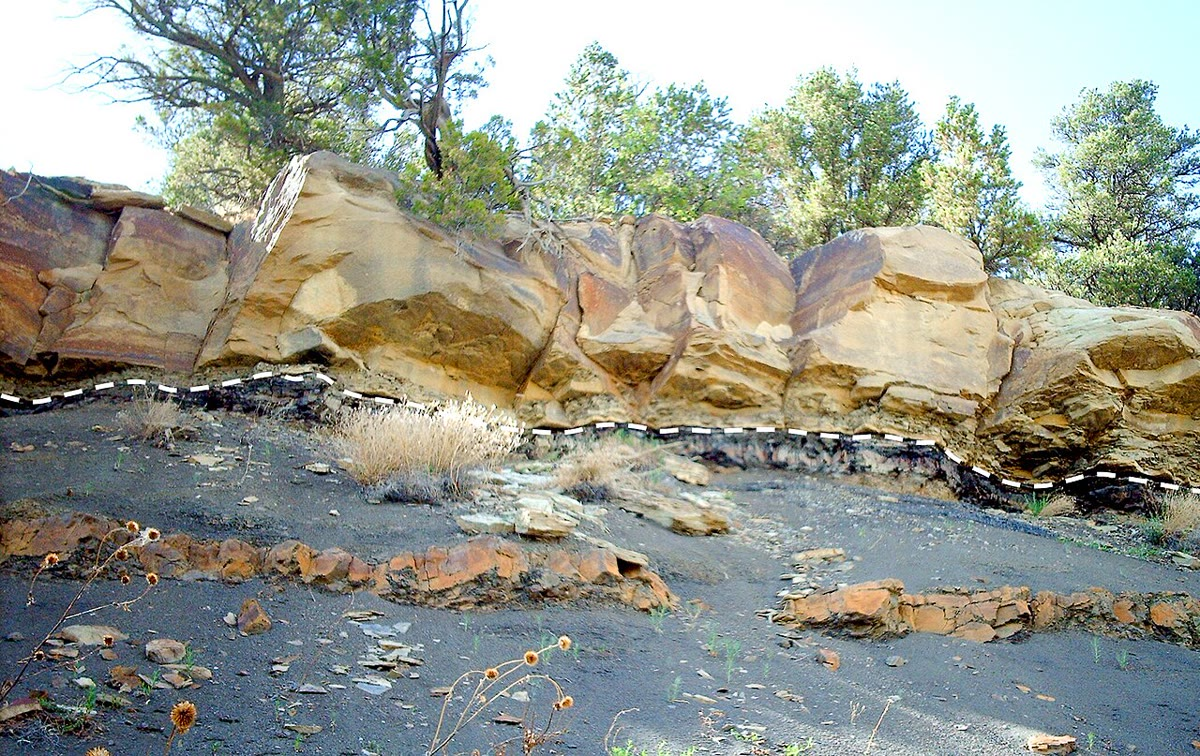
\includegraphics[width=0.78\linewidth]{images/book3/b1-kpg-boundary-trinidad.jpg}

{\small El límite entre el Cretácico y el Paleógeno, marcado por la línea discontinua, en el Parque Estatal del Lago Trinidad, Colorado: arenisca encima, capas oscuras debajo y a lo largo del límite. (Nationalparks, CC~BY-SA~2.5, a través de Wikimedia Commons; la línea discontinua está en el original.)}
\label{fig:b1:stratigraphic-scale:kpg}
\end{omfigure}
% ledger: commons:kt-tlsp

\subsection*{El fin del Pérmico}

La extinción del final del Pérmico fue la pérdida más grave de vida marina y terrestre de los últimos medio millardo de años. En Meishan, en China, la sección que contiene el GSSP de la base del Triásico, cinco capas de ceniza se han datado por el método uranio--plomo sobre circón. Sitúan la extinción entre \qty[uncertainty-mode=separate]{251.941(37)}{\Ma} y \qty[uncertainty-mode=separate]{251.880(31)}{\Ma}: un intervalo de \num[uncertainty-mode=separate]{60 \pm 48} mil años. Un descenso negativo brusco de \qty{3}{\permil} en los isótopos del carbono de los carbonatos lo precede, y el ciclo del carbono siguió inestable durante unos \num{500} mil años.
% ledger: burgess:end-permian, gssp:induan

La base del Triásico, \qty[uncertainty-mode=separate]{251.902(24)}{\Ma}, no se coloca en la extinción, sino en la primera aparición del conodonto \emph{Hindeodus parvus}, un nivel que cae dentro del intervalo de la extinción datado en Meishan. Una extinción es un conjunto de últimas apariciones, que la preservación difumina; una primera aparición bien conocida de una especie traza una línea más nítida. Las causas de las dos extinciones ---un impacto, las grandes provincias de basalto--- son el tema del volumen del año~2.
% ledger: gssp:induan, isg:biostratigraphy, burgess:end-permian

\section{La carta internacional}\label{sec:b1:stratigraphic-scale:chart}

La Carta Cronoestratigráfica Internacional reúne todas las unidades, desde los eonotemas hasta los \omterm{def:b1:stratigraphic-scale:chronostratigraphy}{pisos}, en una sola tabla: sus nombres, la base de cada una en millones de años con su incertidumbre, una marca para cada base definida por un GSSP ratificado, y un color estándar para cada unidad, el de la Comisión para la Carta Geológica del Mundo. La parte fanerozoica, reducida a sus eras y períodos, se dibuja a continuación a partir de los propios valores de la carta.
% ledger: ics:base.Paleozoic, ics:colour.Paleozoic, gssp:count

\begin{omfigure}
\begin{tikzpicture}[font=\footnotesize]
\begin{axis}[y dir=reverse, ymin=0, ymax=538.8, xmin=0, xmax=6.2,
  width=6.6cm, height=11cm, scale only axis, clip=false,
  axis x line=none, axis y line*=left, ytick={0,100,...,500},
  ylabel={edad (\unit{\Ma})}, tick label style={font=\scriptsize}]
  \pgfplotsinvokeforeach{Paleozoic,Mesozoic,Cenozoic,Cambrian,Ordovician,Silurian,Devonian,Carboniferous,Permian,Triassic,Jurassic,Cretaceous,Paleogene,Neogene,Quaternary}{
    \addplot[fill=ics#1, draw=black!70, line width=0.3pt] table[x=x, y=age] {figdata/out/bachelor-1-ics_chart-bar-#1.dat};}
  \addplot[draw=none, nodes near coords, point meta=explicit symbolic,
    every node near coord/.style={anchor=center, rotate=90, font=\scriptsize\bfseries}]
    coordinates {(0.5,395.351) [Paleozoico] (0.5,158.951) [Mesozoico] (0.5,33) [Cenozoico]};
  \addplot[draw=none, nodes near coords, point meta=explicit symbolic,
    every node near coord/.style={anchor=center, font=\scriptsize}]
    coordinates {(2,512.825) [Cámbrico] (2,464.975) [Ordovícico] (2,431.36) [Silúrico] (2,389.24) [Devónico] (2,328.88) [Carbonífero] (2,275.401) [Pérmico] (2,226.651) [Triásico] (2,172.25) [Jurásico] (2,104.55) [Cretácico] (2,44.52) [Paleógeno] (2,12.81) [Neógeno]};
  \addplot[mark=-, mark size=3pt, only marks, nodes near coords, point meta=explicit symbolic,
    every node near coord/.style={anchor=west, xshift=1pt, font=\scriptsize}]
    table[x=x, y=age, meta=lab] {figdata/out/bachelor-1-ics_chart-bases.dat};
  \addplot[only marks, mark=triangle*, mark size=3pt, mark options={rotate=90, fill=omThm, draw=omThm},
    nodes near coords, point meta=explicit symbolic,
    every node near coord/.style={anchor=west, xshift=3pt, font=\scriptsize, text=omThm}]
    coordinates {(4.75,251.902) [fin del Pérmico] (4.75,66) [fin del Cretácico]};
  \node[anchor=south, font=\scriptsize] at (axis cs:2,0) {Cuaternario};
  \node[anchor=west, font=\scriptsize] at (axis cs:3.0,-14) {0};
  \node[anchor=south, font=\scriptsize\itshape] at (axis cs:0.5,-30) {era};
  \node[anchor=south, font=\scriptsize\itshape] at (axis cs:2,-30) {período};
  \node[anchor=south, font=\scriptsize\itshape] at (axis cs:3.5,-30) {base (\unit{\Ma})};
\end{axis}
\end{tikzpicture}

{\small El Fanerozoico en la carta internacional: sus tres eras y doce períodos, a escala, con los colores de la carta, con la edad de la base de cada período (incertidumbres omitidas).
Los triángulos marcan las dos bases que son horizontes de extinción masiva. El Cuaternario, de \qty{2.58}{\Ma} de duración, es la banda delgada de arriba.}
\label{fig:b1:stratigraphic-scale:chart}
\end{omfigure}
% computed in figdata/bachelor-1/ics_chart.py; ledger: ics:base.Cambrian, ics:colour.Cambrian (every ics base and colour row of the eras and periods), burgess:end-permian, alvarez:iridium

Los períodos son muy desiguales (figura de arriba). El Cretácico duró \qty{77.1}{\Myr}, el Neógeno \qty{20.46}{\Myr} y el Cuaternario solo \qty{2.58}{\Myr}; la media de los doce es de \qty{44.9}{\Myr}. La desigualdad es heredada:
los \omterm{def:b1:stratigraphic-scale:chronostratigraphy}{sistemas} se nombraron en \omterm{def:b1:clastic-sediments:sorting}{clasificaciones} antiguas, antes de que ninguna roca se datara en años ---algunos nombres dan una posición (Paleógeno, Neógeno, Cuaternario), algunos una roca (Carbonífero, Cretácico), algunos un pueblo o un lugar (Ordovícico, Silúrico, Devónico, Pérmico)---
y la carta conserva los nombres mientras define sus bases mediante GSSP. Las edades en años proceden de la datación isotópica de rocas volcánicas cercanas a los límites, como las capas de ceniza de Meishan (\cref{ch:b1:radiometric-methods}), interpoladas
como en \cref{prop:b1:stratigraphic-scale:interpolation}; una nueva versión de la carta puede desplazar una edad mientras el GSSP permanece donde está.
% ledger: ics:base.Cretaceous, ics:base.Neogene, ics:base.Quaternary, isg:chronostratigraphy, burgess:end-permian

\begin{dated}{2024}
% ledger: iugs:anthropocene
El Antropoceno, un nombre propuesto en 2001 para un nuevo intervalo marcado por la actividad humana, fue estudiado desde 2009 por un grupo de trabajo de la Subcomisión de Estratigrafía del Cuaternario. A finales de 2023 el grupo propuso una \omterm{def:b1:stratigraphic-scale:chronostratigraphy}{serie} que empieza hacia 1950, con su GSSP en el sedimento del lago Crawford, Ontario. La votación de la subcomisión, cerrada el 4 de marzo de 2024, la rechazó: 4 votos a favor, 12 en contra, 3 abstenciones, 3 miembros sin votar. Los miembros con voto de la Comisión Internacional de Estratigrafía reconocieron la votación. El Antropoceno no es una unidad de la carta; sigue siendo un término informal, muy usado.
\end{dated}

\section{Ejercicios}

\begin{exercise}[$\star$]\label{exo:b1:stratigraphic-scale:1}
Dígase si cada nombre es el de una \omterm{def:b1:stratigraphic-scale:lithostratigraphy}{unidad litoestratigráfica}, biostratigráfica, cronoestratigráfica o geocronológica, y dése su rango cuando lo tiene: (a)~el \omterm{def:b1:stratigraphic-scale:chronostratigraphy}{Sistema} Jurásico; (b)~la \omterm{def:b1:stratigraphic-scale:lithostratigraphy}{Formación} de Lutita de Mardon; (c)~el Cretácico Inferior; (d)~la zona de \emph{Hindeodus parvus}; (e)~el \omterm{def:b1:stratigraphic-scale:chronostratigraphy}{piso} Daniense; (f)~la Época del Paleoceno; (g)~un \omterm{def:b1:stratigraphic-scale:lithostratigraphy}{miembro} de arenisca de la Lutita de Mardon.
% ledger: isg:lithostratigraphy, isg:biostratigraphy, isg:chronostratigraphy
\end{exercise}

\begin{exercise}[$\star$]\label{exo:b1:stratigraphic-scale:2}
Con las bases de las eras en la figura de la carta (las del Cámbrico, del Triásico y del Paleógeno), calcúlese la duración del Paleozoico, del Mesozoico y del Cenozoico, y la parte del Fanerozoico que representa cada una. ¿Qué parte del tiempo desde la base del Hadeico, \qty{4567}{\Ma}, representa todo el Fanerozoico?
% ledger: ics:base.Paleozoic, ics:base.Mesozoic, ics:base.Cenozoic, ics:base.Hadean
\end{exercise}

\begin{exercise}[$\star$]\label{exo:b1:stratigraphic-scale:3}
Un acantilado muestra, de abajo arriba: estratos A, B, C y D, inclinados \ang{40}; un dique E que corta de A a D; una superficie de erosión que corta la cima de D y el dique; estratos horizontales F y G encima; una falla que desplaza de A a F pero no a G. Ordénense los sucesos y nómbrese el principio que justifica cada paso.
\end{exercise}

\begin{exercise}[$\star$]\label{exo:b1:stratigraphic-scale:4}
Dos capas de ceniza separadas \qty{30}{m} en una lutita se datan en \qty{85.40}{\Ma} (la inferior) y \qty{84.60}{\Ma} (la superior). La primera aparición de un \omterm{def:b1:stratigraphic-scale:biozone}{fósil guía} yace \qty{12}{m} por encima de la ceniza inferior. Calcúlese la tasa de acumulación y la edad de la primera aparición, suponiendo que la tasa es constante.
\end{exercise}

\begin{exercise}[$\star\star$]\label{exo:b1:stratigraphic-scale:5}
En una sección, cuatro taxones tienen los rangos (alturas en metros): A 0--34, B 12--50, C 26--62, D 41--70. (a)~Dibújese el diagrama de rangos. (b)~Dese la extensión y el espesor de la \omterm{def:b1:stratigraphic-scale:biozone}{zona de rangos} concurrentes de B y C, y de la \omterm{def:b1:stratigraphic-scale:biozone}{zona de intervalo} entre las primeras apariciones de B y D. (c)~En una segunda sección, B se encuentra de 3 a 15~m y C de 9 a 22~m, y no se sabe nada más. ¿Qué límites de zona de (b) pueden reconocerse allí, y cuáles no? ¿Qué horizontes pueden correlacionarse entre las dos secciones con más seguridad?
\end{exercise}

\begin{exercise}[$\star\star$]\label{exo:b1:stratigraphic-scale:6}
Durante una transgresión la línea de costa avanzó tierra adentro a \qty{20}{km} por millón de años. (a)~¿En cuánto difiere la edad de la cima de la arenisca de la línea de costa entre dos pozos separados \qty{60}{km} según la dirección de la transgresión? (b)~Una ceniza cae un millón de años después de que la línea de costa pasara el pozo más marino, donde el lodo de mar adentro se acumula a \qty{30}{m} por millón de años. ¿A qué altura por encima de la cima de la arenisca se encuentra allí el estrato de ceniza? (c)~¿Dónde estaba la línea de costa cuando cayó la ceniza? ¿Se encuentra la ceniza por encima o por debajo de la arenisca en el pozo tierra adentro, y por qué puede no encontrarse allí en absoluto? Explíquese con un esbozo.
\end{exercise}

\begin{exercise}[$\star\star$]\label{exo:b1:stratigraphic-scale:7}
(a)~Calcúlese, en por ciento, la incertidumbre relativa de las edades de las bases del Lochkoviense (\qty[uncertainty-mode=separate]{419.62(136)}{\Ma}) y del Induense (\qty[uncertainty-mode=separate]{251.902(24)}{\Ma}).
Sugiérase por qué difieren tanto. (b)~A partir de las dos edades que encuadran la extinción del final del Pérmico en Meishan, \qty[uncertainty-mode=separate]{251.941(37)}{\Ma} y
\qty[uncertainty-mode=separate]{251.880(31)}{\Ma}, recalcúlese la duración de la extinción y su incertidumbre, suponiendo independientes los dos errores. Compárese con los publicados
\num[uncertainty-mode=separate]{60 \pm 48} mil años.
% ledger: ics:base.Devonian, gssp:induan, burgess:end-permian
\end{exercise}

\begin{exercise}[$\star\star$]\label{exo:b1:stratigraphic-scale:8}
Tómese el \omterm{def:b1:comparative-planetology:small-bodies}{asteroide} de 1980 como una esfera de \qty{10}{km} de diámetro, de densidad \qty{3000}{kg.m^{-3}} (valor supuesto), que lanza a la atmósfera 60 veces su masa en polvo. (a)~Calcúlense la masa del
\omterm{def:b1:comparative-planetology:small-bodies}{asteroide} y la del polvo. (b)~Repártase el polvo uniformemente sobre la Tierra (diámetro \qty{12756}{km}): ¿qué masa cae sobre cada metro cuadrado? (c)~Depositado con una densidad de
\qty{2500}{kg.m^{-3}}, ¿qué espesor tiene la capa? (d)~Repítase (c) para diámetros de \qty{6}{km} y \qty{14}{km}, el intervalo de la estimación. Compárese con el espesor de la arcilla del límite en el GSSP del Daniense.
% ledger: alvarez:iridium, planet:Earth.diameter, gssp:danian
\end{exercise}

\begin{exercise}[$\star\star$]\label{exo:b1:stratigraphic-scale:9}
(a)~En una sección condensada donde el sedimento se acumuló a \qty{2}{m} por millón de años, ¿qué espesor tiene el intervalo de \num{60} mil años de la extinción del final del Pérmico? ¿Qué espesor tendría para
las duraciones más corta y más larga permitidas por su incertidumbre? (b)~En una sección marina profunda que se acumula a \qty{10}{m} por millón de años, ¿qué espesor tiene el intervalo de \num{32000} años
dentro del cual el impacto y el límite K--Pg son sincrónicos? (c)~¿Qué dicen estas cifras sobre el muestreo de una sección para estudiar una extinción?
% ledger: burgess:end-permian, renne:kpg
\end{exercise}

\begin{exercise}[$\star\star\star$]\label{exo:b1:stratigraphic-scale:10}
Una llanura costera tiene una pendiente de $1$ por $2000$ y el \omterm{def:b1:diagenesis-basins:eustasy}{nivel relativo del mar} sube a \qty{10}{m} por millón de años. (a)~Con \cref{prop:b1:stratigraphic-scale:transgression}, ¿con qué rapidez
se desplaza tierra adentro la línea de costa, y en cuánto difiere la edad de la cima de la arenisca de la línea de costa entre dos pozos separados \qty{30}{km}? (b)~Ahora se entrega sedimento a la costa, que
construye la llanura costera hacia arriba $a$ metros por millón de años en la línea de costa. Demuéstrese que la línea de costa se desplaza tierra adentro a $(R - a)/s$ mientras $a < R$. ¿Qué ocurre cuando
$a > R$? (c)~Explíquese por qué una cima de arenisca cuya edad cambia un millón de años puede parecer, en un solo acantilado, exactamente una superficie de igual edad.
\end{exercise}

\begin{exercise}[$\star\star\star$]\label{exo:b1:stratigraphic-scale:11}
Dos capas de ceniza yacen a \qty{10}{m} y a \qty{50}{m} en una sección y se datan en \qty[uncertainty-mode=separate]{100.50(5)}{\Ma} y \qty[uncertainty-mode=separate]{99.70(3)}{\Ma}. (a)~Interpólese la edad de un nivel a
\qty{25}{m} y su incertidumbre con \cref{prop:b1:stratigraphic-scale:interpolation}. (b)~¿Dónde, entre las dos cenizas, es mínima la incertidumbre? Hállese el valor de $f$ que minimiza $\sigma_t$, y el mínimo.
(c)~Demuéstrese que $\sigma_t$ nunca supera la mayor de $\sigma_1$ y $\sigma_2$ entre las dos capas.
\end{exercise}

\begin{exercise}[$\star\star\star$]\label{exo:b1:stratigraphic-scale:12}
Un pozo atraviesa una lutita uniforme. Una ceniza datada en \qty{30.0}{\Ma} yace a \qty{1000}{m} de profundidad y una ceniza datada en \qty{29.0}{\Ma} a \qty{200}{m}; un límite de \omterm{def:b1:stratigraphic-scale:chronostratigraphy}{piso} yace a \qty{600}{m}. (a)~Interpólese
su edad a partir de las profundidades. (b)~Los granos, no los poros, llegaron a una tasa constante. Usando la lutita de \cref{tab:b1:diagenesis-basins:athy} y \cref{prop:b1:diagenesis-basins:solid}, calcúlese
el espesor sólido entre cada ceniza y el límite, e interpólese de nuevo la edad en proporción a él. (c)~¿En cuántos miles de años difieren las dos estimaciones, y cuál es la mejor?
% ledger: pybacktrack:compaction
\end{exercise}

\section{Problema: correlación de tres secciones a través de una cuenca}

\begin{problem}[{Problema de fin de semana --- cómo se combinan los fósiles, las capas de ceniza y una arenisca diacrónica para datar un límite de piso}]
\label{pb:b1:stratigraphic-scale:1}
% values: calc/ch24.py; the basin, its sections, its taxa (Vardenoceras and Ostreola) and its ash ages are invented
Se levantan tres secciones a lo largo de una línea a través de una cuenca inventada: A al oeste, B \qty{25}{km} al este de A, y C \qty{20}{km} al este de B. En cada una, la Arenisca de Kell está
cubierta por la Lutita de Mardon. Las alturas están en metros sobre la base de cada sección:
\begin{center}
\small
\begin{tabular}{lccc}
\hline
 & A & B & C \\
\hline
total de espesor registrado                       & 80.0 & 66.0 & 32.0 \\
cima de la Arenisca de Kell                    & 45.0 & 20.0 & 6.0 \\
capa de ceniza 1 (datada \qty[uncertainty-mode=separate]{152.40(4)}{\Ma})       & 5.0  & 8.0  & 3.0 \\
capa de ceniza 2 (datada \qty[uncertainty-mode=separate]{151.20(4)}{\Ma})       & 71.0 & 56.0 & 27.0 \\
primera aparición de \emph{Vardenoceras medium} & 36.6 & 31.2 & 14.8 \\
primera aparición de \emph{Vardenoceras ultimum} & 65.8 & 52.0 & 24.8 \\
última aparición de \emph{Vardenoceras primum}   & 49.0 & 40.0 & 19.0 \\
\hline
\end{tabular}
\end{center}
\emph{V.~primum} se encuentra desde la base de todas las secciones. El bivalvo \emph{Ostreola} solo se encuentra en la Arenisca de Kell, en las tres secciones. Se definen tres \omterm{def:b1:stratigraphic-scale:biozone}{zonas de intervalo}: la zona~1 hasta la primera aparición de \emph{V.~medium}, la zona~2 hasta la de \emph{V.~ultimum}, la zona~3 por encima. Un límite de \omterm{def:b1:stratigraphic-scale:chronostratigraphy}{piso} se define, en su GSSP situado en otro lugar, por la primera aparición de \emph{V.~medium}.

\medskip
\noindent\textbf{Parte I --- Biozonas.}
\begin{enumerate}
  \item Dibújense las tres secciones una al lado de otra con una escala vertical común, con la Arenisca de Kell, las capas de ceniza y los límites de zona.
  \item Dése el espesor de la zona~2 en cada sección, y el espesor de la parte de la zona~3 registrada.
  \item ¿Por qué no puede situarse la base de la zona~1 en ninguna de las tres secciones?
  \item ¿Por qué \emph{Ostreola} es un mal \omterm{def:b1:stratigraphic-scale:biozone}{fósil guía}, por común que sea?
  \item ¿En qué zona cae la última aparición de \emph{V.~primum} en cada sección? ¿Podría servir como cuarto límite de zona?
  \item Correlaciónense las secciones por las primeras apariciones de \emph{V.~medium} y \emph{V.~ultimum}. ¿Qué sugiere el cociente de los espesores de la zona~2?
\end{enumerate}

\noindent\textbf{Parte II --- La Arenisca de Kell.}
\begin{enumerate}[resume]
  \item ¿En qué zona yace la cima de la Arenisca de Kell en cada sección?
  \item ¿Es la cima de la Arenisca de Kell una superficie de igual edad? ¿En qué sentido se desplazó la línea de costa, y qué clase de suceso es este?
  \item La capa de ceniza~1 yace en la Arenisca de Kell en las tres secciones, la capa de ceniza~2 en la Lutita de Mardon. ¿Por qué las capas de ceniza son mejores líneas de tiempo que el límite de \omterm{def:b1:stratigraphic-scale:lithostratigraphy}{formación}?
  \item ¿Cuál de los principios de \cref{def:b1:stratigraphic-scale:principles} justifica seguir una sola capa de ceniza de A a C?
\end{enumerate}

\noindent\textbf{Parte III --- Tasas.}
\begin{enumerate}[resume]
  \item Calcúlese la tasa de acumulación entre las dos capas de ceniza en cada sección, en metros por millón de años.
  \item Sugiérase por qué la tasa disminuye de A a C.
  \item ¿Cuántos años representa una muestra de \qty{10}{cm} de espesor en cada sección? ¿Qué sección da la resolución temporal más fina?
  \item Suponiendo tasas constantes, calcúlese la edad de la cima de la Arenisca de Kell en cada sección.
  \item Calcúlese la velocidad de la línea de costa entre C y B y entre B y A, en kilómetros por millón de años. ¿Se aceleró o se frenó la transgresión?
  \item Calcúlese la edad de la primera aparición de \emph{V.~ultimum} en cada sección.
  \item ¿Concuerdan las tres edades de la pregunta~16 dentro de la incertidumbre de las dataciones de las cenizas? ¿Qué dice esto sobre la primera aparición?
\end{enumerate}

\noindent\textbf{Parte IV --- La edad del límite.}
\begin{enumerate}[resume]
  \item Interpólese, en cada sección, la edad de la primera aparición de \emph{V.~medium}.
  \item Calcúlese la incertidumbre de cada edad a partir de las incertidumbres de las dataciones de las cenizas con \cref{prop:b1:stratigraphic-scale:interpolation}.
  \item Calcúlense la media de las tres edades y su dispersión. ¿Es la dispersión mayor o menor que la incertidumbre de la pregunta~19?
  \item En la sección~A la primera aparición de \emph{V.~medium} yace en la Arenisca de Kell, y en B y C en la Lutita de Mardon. ¿Cómo podría un cambio de litología entre las capas de ceniza sesgar la interpolación en A?
  \item ¿Cuál de las tres secciones sería el mejor \omterm{def:b1:stratigraphic-scale:gssp}{estratotipo de límite}, y por qué? ¿Cuál sería el peor?
  \item ¿Cuánto duró la zona~2?
  \item ¿Cuál es la edad interpolada del límite?
\end{enumerate}
\end{problem}
